% this file is called up by thesis.tex
% content in this file will be fed into the main document

%: ----------------------- name of chapter  -------------------------
\chapter{Network Design} % top level followed by section, subsection


%: ----------------------- paths to graphics ------------------------

% change according to folder and file names
\ifpdf
    \graphicspath{{X/figures/PNG/}{X/figures/PDF/}{X/figures/}}
\else
    \graphicspath{{X/figures/EPS/}{X/figures/}}
\fi

%: ----------------------- contents from here ------------------------

\section{Overview}

Chpater 4 mainly discuss the network design of the HCMP Player,  
focus will be on illustrating design decision behind the network function of    
HCMP Player, A full list of network API will be given, by which any other 
HCMP componets can use to communicate with HCMP Player through network.   
Apart from network API, chapter 4 also discuss how HCMP player establish a 
connection with remote server at first place. In real implementation, the HCMP Player 
use zeromq library to facilitate network devleopment. Zeromq library 
integrate several
different ways for communication between nodes within network range.
We will briefly discuss each method, together with its pros and cons, and 
its usage inside the HCMP Player.

\section{Conductor and Player}
In network module of HCMP Player, 3 kinds of design pattern is mainly used. The 
request \& reply design pattern is the most commonly used one, it is used in 
building connection between remote server
and HCMP Player. After connection has been established, the remote server and
HCMP Player will adapt another kind of pattern, observer pattern. 

\subsection{Request \& Reply Pattern}
The request and reply pattern is the most basic pattern used in network 
communication. Just as its name suggests, the server send request to client, 
after receving the request, client handle the request and send reply to 
server. This pattern is heavily used in remote procedure call (RPC) programming 
model, for example, the caller object can invoke some methods from callee 
object regardless of callee object is stored in local machine memory or
memory space in a remote machine. The most typical use is in web programming, 
where user press a button, this event eventually invoke a method in server-side, 
after some computation, the server reply with result to webpage. In most cases, 
the request \& reply pattern
rely on the feature of TCP to reliably deliver the message. 

Figure 4.1 indicate how this pattern works in HCMP Player. In HCMP Player, 
when user try to establish the connection with remote  
server, it will send request and wait for its reply. A timeout limit is set to 
avoid waiting for too long. If connect to a remote server failed, the HCMP Player
will ``rollback'' to stand-alone mode.
\begin{figure}[H]
\center{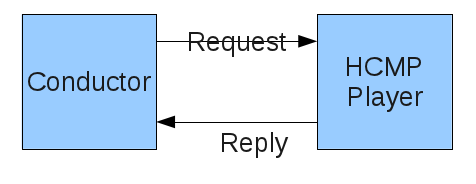
\includegraphics[width=0.55\linewidth]{4/3.png}}
\caption{Request-Reply Pattern}
\label{fig:speciation}
\end{figure}

\subsection{Observer Pattern}
In observer pattern, there is an subject object, the subject object  maintains 
a list of its dependents, which are called observers, and notifies them 
automatically of any state changes, usually by calling one of their methods. Figure
\begin{figure}[H]
\center{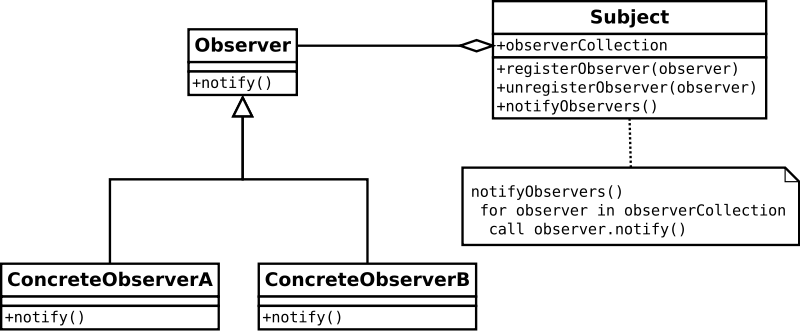
\includegraphics[width=0.8\linewidth]{4/5.png}}
\caption{UML Diagram of Observer Pattern}
\label{fig:speciation}
\end{figure}

After connection has been built, the remote server and the HCMP Player form a 
observer-pattern relationship, where remote server is the subject and HCMP Player 
is dependent. Firstly, the HCMP Player try to use a RPC call to register into 
remote server dependents list, then it wait for reply from the remote server. In real 
implementation, the conductor is in remote server part and resposible
for synchronizing all the HCMP Players. Each conductor will maintain list of HCMP Players
, this list will be updated once old player become obselete, or new player join in.
Figure 4.3 illustrate observer pattern in HCMP Player.  
\begin{figure}[H]
\center{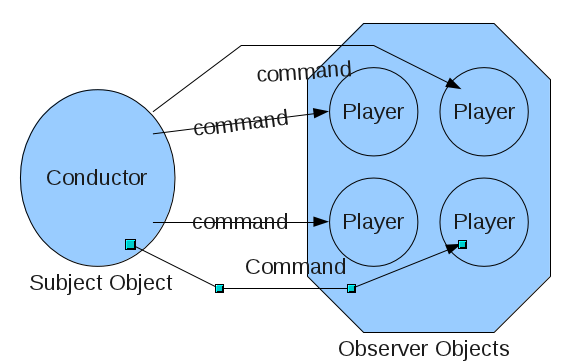
\includegraphics[width=0.65\linewidth]{4/2.png}}
\caption{Observer Pattern}
\label{fig:speciation}
\end{figure}

\subsection{Push \& Pull Pattern}
In order to monitor the status of each HCMP Player, each registered HCMP Player 
need to periodically push ``heart beat'' message to remote server. 
The remote server set a count down timer for each HCMP Player currently 
connected to server. It  
then periodically pull message and then reset according HCMP Player's timer. 
If there exist a timer reach 
zero, then remote server will further send confirm message, temporarily deregsiter 
this HCMP Plyaer from dependent list. Figure 4.4 indicate how push \& pull pattern 
used in HCMP Player.

\begin{figure}[H]
\center{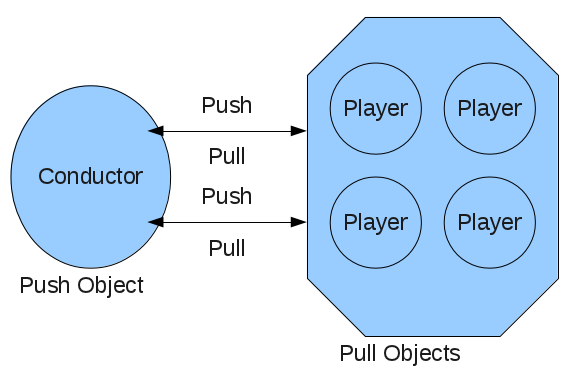
\includegraphics[width=0.65\linewidth]{4/4.png}}
\caption{Push \& Pull Pattern}
\label{fig:speciation}
\end{figure}

\section{Network Programming Interface}
The programming interface defined below is used for communication 
between remote server and HCMP Player. Any external exponent that  
follows these APIs is able to communicate and take control of the 
HCMP Player.
The GUI component is responsible for receving all the network request. 
Imagine a situation where remote server   
try to start command to all HCMP players. The remote server send start 
request to all HCMP players in its dependent list.
Once the request is sucessfully delivered, the GUI of HCMP player will 
receive and handle the request, after parsing the request string, 
it map and invoke the internal API, then send the request to player engine 
through message queue. Once player engine read from message queue and
begin to schedule the first midi note, the HCMP Player start playing.

\begin{figure}[H]
\center{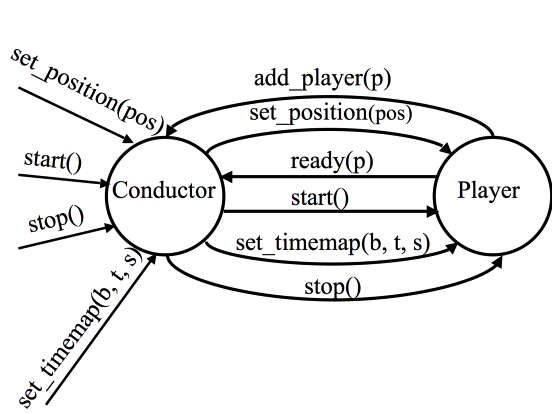
\includegraphics[width=0.5\linewidth]{3/1.png}}
\caption{HCMP Player Network API}
\label{fig:speciation}
\end{figure}
Figure 4.5 illustrate how conductor coordiate with HCMP Player, all the  
related APIs are list below \\

From remote server to HCMP Player
\begin{itemize}
  \item \texttt{play - start playing}  
  \item \texttt{stop - stop playing}
  \item \texttt{pause - pause current playing}
  \item \texttt{update\_time\_map - send new time map to player}  
  \item \texttt{set\_position - set play position to the given parameter}
\end{itemize}

From HCMP Player to remote server
\begin{itemize}
  \item \texttt{play\_all - inform the remote server to play}  
  \item \texttt{stop\_all - inform the remote server to stop}  
  \item \texttt{ready - inform the remote server is ready to play}
  \item \texttt{position - inform remote server to begin from specified position}
\end{itemize}
